%\documentclass[10pt, conference, compsocconf]{IEEEtran}
\documentclass[a4paper]{sbgames}               

\usepackage{times}
\usepackage{graphicx}
\usepackage{amsmath,amssymb,amsthm,siunitx}
\usepackage[brazil,american]{babel}
\usepackage[utf8]{inputenc}
\usepackage{hyperref}
\usepackage{float}

%% use this for zero \parindent and non-zero \parskip, intelligently.
\usepackage{parskip}

%% the 'caption' package provides a nicer-looking replacement
%\usepackage[labelfont=bf,textfont=it]{caption}

\usepackage{url}
\renewcommand{\rmdefault}{ptm} % Usa a fonte Times New Roman
\renewcommand{\sfdefault}{phv} % Usa a fonte Helvetica
\renewcommand{\ttdefault}{pcr} % Usa a fonte Courier

\usepackage{sectsty}
\sectionfont{\fontsize{14}{15}\selectfont} % Define o tamanho da fonte das seções
\subsectionfont{\fontsize{14}{13}\selectfont} % Define o tamanho da fonte das subseções

\begin{document}

%% Paper title.
\title{Badly Programmed Ice Cream}


% \author{\IEEEauthorblockN{Autor1, Autor2, and Autor3}
% \IEEEauthorblockA{Dept. of Computer Science\\
% University of Brasilia\\ Brasilia, Brazil\\
% Email: \{autor1, autor2\}@gmail.com autor3@hotmail.com}
% }

 \author{ Arthur Araújo - 232000472
         \hspace{28pt} Arthur Silva - 232000490
         \hspace{28pt} João Carlos - 232009511 \\
         \vspace{0pt} \\
         {University of Brasília, Dept. of Computer Science, Brazil} }
        
\vspace{1.5cm}


% make the title area
\maketitle

% Abstract section.

\begin{abstract}
O projeto "Badly Programmed Ice Cream" foi criado como um remake do jogo Bad Ice Cream feito em Assembly RISC-V utilizando o RARS como ferramenta de desenvolvimento. O projeto foi desenvolvido durante as aulas da disciplina de Introdução a Sistemas Computacionais. RISC-V é uma arquitetura de conjunto de instruções (ISA) baseada em princípios de design de processadores de redução de conjunto de instruções (RISC). Ela é caracterizada por ser livre e aberta, o que significa que seu design está disponível publicamente e pode ser usado livremente por qualquer pessoa ou organização. Foi desenvolvida na Universidade da Califórnia, em Berkeley, e é amplamente reconhecida por sua flexibilidade e eficiência.
\end{abstract}


\section{Introdução}
\label{sec:introducao}


"Bad Ice-Cream" é um jogo de arcade desenvolvido pela Nitrome, lançado em 10 de Dezembro de 2010. No jogo, os jogadores controlam um personagem que deve coletar frutas em um labirinto enquanto evita inimigos. O objetivo é coletar todas as frutas para completar o nível. O jogo é conhecido por seu estilo de arte pixelizada e jogabilidade simples, mas desafiadora.
No jogo original, o jogador deve escolher um dos sorvetinhos para controlar, sendo capaz de criar blocos de gelo para bloquear inimigos ou abrir caminho através do labirinto, mas também devem evitar que os inimigos quebrem os blocos de gelo ou os atinjam diretamente. Novos desafios e elementos são introduzidos ao longo das fases, tornando cada nível mais complexo e exigindo estratégia e habilidade para serem concluídos.


\begin{figure}[htb]
  \begin{center}
   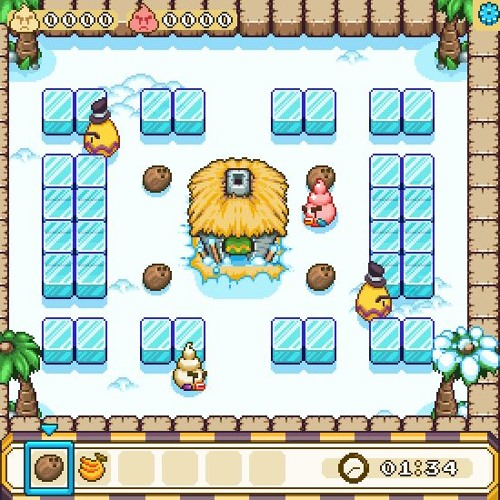
\includegraphics[width=1.0\linewidth]{./Figures/mapaoriginal.jpg}
  \end{center}
  \caption{Jogo original Bad Ice Cream}
  \label{fig:01}
\end{figure}


Na seção \ref{sec:Metodologia} será apresentada a metodologia utilizada. A seção \ref{sec:Resultados} apresenta os resultados obtidos. A seção \ref{sec:Conclusao} conclui este trabalho.

\section{Metodologia}
\label{sec:Metodologia}

Inicialmente, o projeto foi desenvolvido no RARS, apresentado pelo professor Lamar. Contudo, durante o semestre, atualizações foram feitas e a testagem passou a ser feita com a ferramenta \href{https://github.com/LeoRiether/FPGRARS}{FPGRARS} criada pelo ex-aluno Leonardo Riether. A ferramenta facilita a execução e garante uma velocidade superior em comparação ao montador original RARS.

De maneira análoga aos projetos de alunos anteriores, foi implementado um sistema baseado em matrizes, as quais determinam o comportamento posicional do jogador, como também dos inimigos e dos coletáveis. 
\subsection{Planejamento}{
\label{sec:planejamento} 


Toda comunicação durante o desenvolvimento do projeto foi realizada via Discord e Whatsapp. O projeto foi iniciado no dia 12/11 e finalizado no dia 21/12. Ao longo de cada semana, houveram reuniões para organização e definição de tarefas semanais. Para o versionamento de código, foi utilizado o GitHub, o qual possibilitou uma melhora significativa na organização e implementação de cada etapa do jogo.

Cada sprite utilizada para representação visual no jogo foi feita em conjunto, caracterizada pelas artes do aluno Arthur Araújo.
}

\begin{figure}[htb]
  \begin{center}
   
\includegraphics[width=1.0\linewidth]{./Figures/spritezinhas.png}
  \end{center}
  \caption{Sprites do player e do inimigo}
  \label{fig:01}
\end{figure}

\subsection{Renderização}
\label{sec:render}

Para renderizar uma imagem no bitmap display do RARS/FPGRARS, foi necessário entender como os dados são interpretados. O bitmap consiste em dois grandes vetores de bytes, cada um representando uma camada de cor na tela. Cada byte do vetor codifica uma cor específica, e a tela tem uma resolução de 320x240 pixels (resolução 4:3). A interpretação dos dados do bitmap é feita de forma sequencial, começando pelo primeiro byte (pixel) na quina superior esquerda da tela e avançando ordenadamente até atingir a quina inferior direita, pulando para a próxima linha a cada 320 pixels.
Nesse viés, com base no entendimento do funcionamento do bitmap display, e no tutorial feito pelo ex-aluno \href{https://www.youtube.com/watch?v=2BBPNgLP6_s}{Davi Paturi}, foi possível implementar o sistema inicial de renderização do mapa e do player.

\begin{figure}[H]
  \centering
  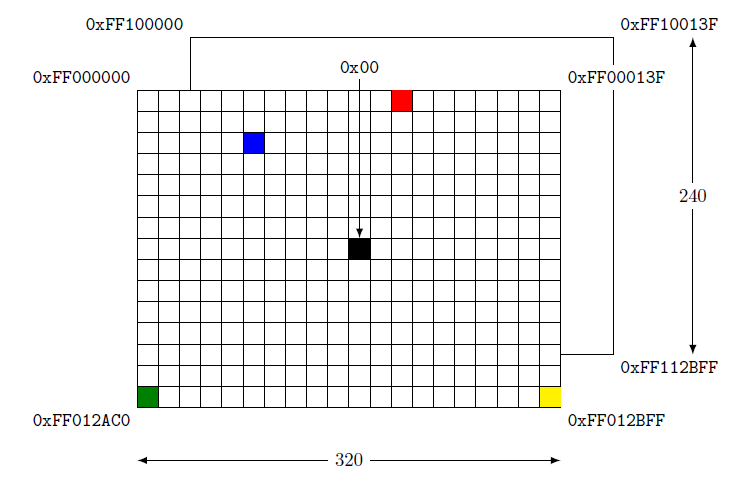
\includegraphics[width=1.0\linewidth]{./Figures/bitmapdisplay.png}
  \caption{Funcionamento do bitmap display}
  \label{fig:01}
\end{figure}

\subsection{Movimentação}{
\label{sec:mov}

Para a movimentação, usamos a chamada do
teclado para definir a direção, sendo: a = esquerda, d = direita, s = baixo e w = cima. Desse modo, utilizamos endereços  que vão verificar a colisão e calcular a nova
posição do personagem, armazenando em
uma .half, enquanto a posição antiga será sobreposta pelo tile de chão.
}

\begin{figure}[H]
  \centering
  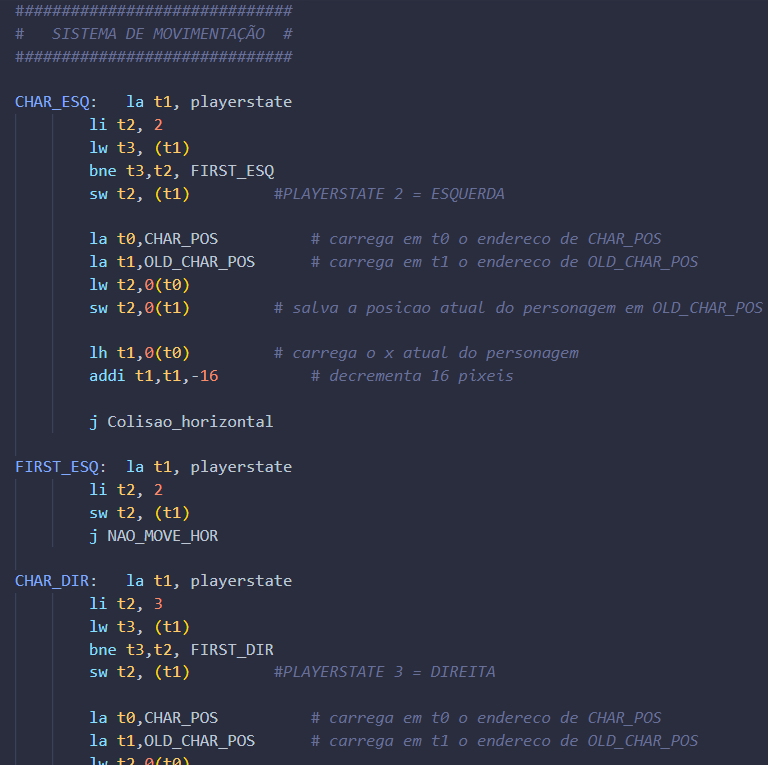
\includegraphics[width=1.0\linewidth]{./Figures/movimentacao.png}
  \caption{Trecho de código do sistema de movimentação}
  \label{fig:01}
\end{figure}

\subsection{Colisão}{
\label{sec:colid}

No sistema de colisão, desenvolvemos uma
matriz (320x240). Na matriz, os índices 0 e 1 representam respectivamente o caminho do chão e dos blocos de parede. Os coletáveis são representados por 2 e o gelo pelo número 3. O inimgo estático da fase inicial é representado pelo 4.
Nesse viés, se a posição pretendida pelo usuário
na movimentação do personagem
corresponder ao número 1 na matriz, a
posição não é alterada. Caso contrário, o personagem é movimentado na direção desejada usando a lógica das
teclas pressionadas, garantindo a colisão com inimigos e coletáveis no bitmap display. 
}

\begin{figure}[H]
  \begin{center}
   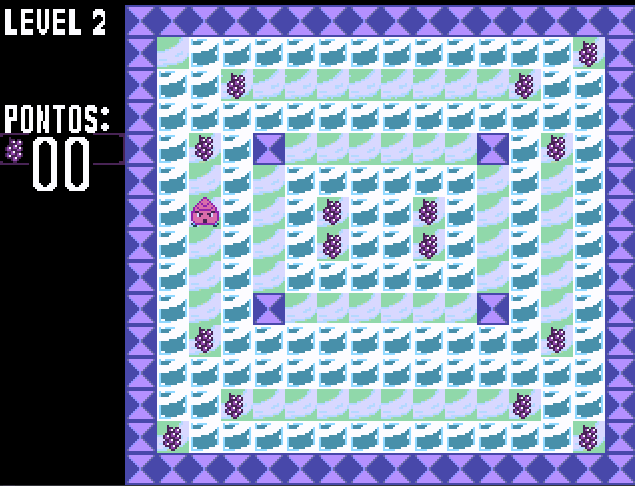
\includegraphics[width=1.0\linewidth]{./Figures/fase2.PNG}
  \end{center}
  \caption{Fase 2 em jogo}
  \label{fig:04}
\end{figure}

\begin{figure}[H]
  \begin{center}
   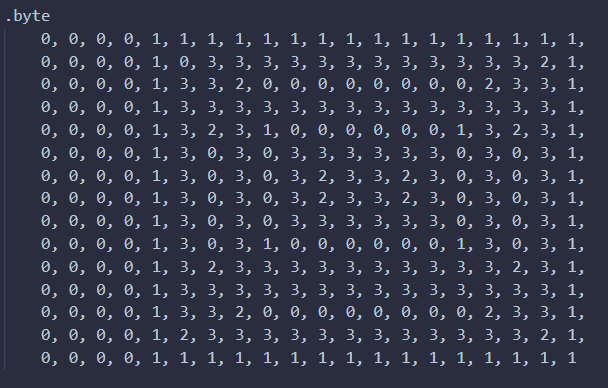
\includegraphics[width=1.0\linewidth]{./Figures/matrizlevel2.PNG}
  \end{center}
  \caption{Matriz de representação da fase 2}
  \label{fig:05}
\end{figure}

\subsection{Ataque}{
\label{sec:att}

A mecânica de ataque funciona de maneira semelhante à movimentação e também está localizada no mesmo script "movement.s". A cada frame, o programa verifica se o jogador pressionou a tecla "J" e, caso afirmativo, direciona o programa para uma sub-rotina que realiza os cálculos para o movimento "especial" do jogador. Primeiramente, é verificada a variável "playerstate", que define para qual lado o jogador está olhando, e redireciona para o código correspondente que imprime os blocos na direção correta. Em seguida, ele usa a variável CHAR-POS e calcula a coordenada exata do bloco respectivo em frente ao jogador. Se o caminho para o ataque estiver livre, o botão "J" cria uma fileira de blocos até encontrar um tile diferente de "0" (livre) na matriz da fase, atualizando toda a fileira na matriz com o tile "3" (gelo). Se o caminho tiver gelo, o ataque quebra a fileira inteira de gelo (3) e reposiciona o caminho livre (0) na matriz. Por fim, se o tile ao lado do jogador for uma parede comum (1), o ataque não é realizado.
}
\begin{figure}[H]
  \begin{center}
   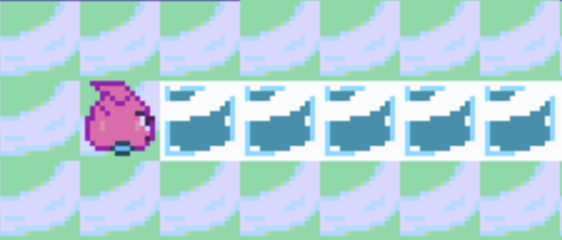
\includegraphics[width=1.0\linewidth]{./Figures/ataque.PNG}
  \end{center}
  \caption{Player realizando o ataque}
  \label{fig:05}
  \end{figure}

\subsection{Música}{
\label{sec:music}

Para a transposição da música de abertura para a forma interpretada em assembly, utilizamos o Hooktheory. Nesse contexto, organizamos as notas musicais e suas durações nessa ordem, representadas por números conforme a interpretação da interface. Os efeitos sonoros foram criados como parte dos testes, nos quais experimentamos os instrumentos disponíveis no próprio RARS em diferentes alturas. Esses testes nos permitiram identificar quais sons poderiam ser associados aos efeitos sonoros desejados. Adicionalmente, incluímos uma música de encerramento para quando a vitória é alcançada.
}

 \begin{figure}[H]
  \begin{center}
   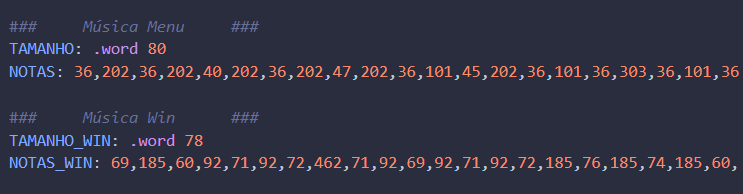
\includegraphics[width=1.0\linewidth]{./Figures/musicas.PNG}
  \end{center}
  \caption{Código da música de abertura}
  \label{fig:05}
  \end{figure}
\newpage

\section{Resultados Obtidos}
\label{sec:Resultados}

Apesar de algumas dificuldades enfrentadas durante o processo de desenvolvimento, é válido afirmar que obtivemos um resultado final geral satisfatório em relação ao projeto. De uma forma simples, a jogabilidade foi aplicada com todas as ferramentas disponibilizadas pelo Assembly RISC-V. Seguem abaixo alguns problemas e desafios que enfrentamos:

\begin{itemize}
    \item A dificuldade inicial foi entender como começar, qual o primeiro passo? A partir dos vídeos de ex-alunos e algumas monitorias, essa etapa foi vencida.
    
    \item Logo em seguida, nossa dificuldade era implementar os coletáveis e impedir que o jogador "quebrasse" o jogo invadindo regiões que não devia, problema que foi solucionado com a criação da matriz de representação.
    
    \item Implementar um inimigo inteligente no RARS foi um desafio que infelizmente não foi possível concluir devido ao tempo insuficiente conforme a entrega final se aproximava.
    
    \item A mecânica do gelo foi um grande desafio, visto que gerava muitos bugs, alguns deles ainda ocultos.
\end{itemize}





\section{Conclusão}
\label{sec:Conclusao}

Desse modo, é visível que o projeto não foi uma tarefa fácil para alunos do primeiro semestre, e, apesar das dificuldades, o resultado foi muito gratificante. Desde o início, sabiamos que desenvolver um jogo em uma linguagem de baixo nível seria uma tarefa árdua. Além disso, o aprendizado foi coletivo e guiado por todos os conteúdos e materiais disponibilizados em inúmeras fontes, como repositórios antigos do github, slides do professor e vídeos escondidos no youtube.

\begin{figure}[H]
  \begin{center}
   
\includegraphics[width=1.0\linewidth]{./Figures/GameOver.PNG}
  \end{center}
  \caption{Tela de Game Over}
  \label{fig:05}


\vspace{1.5cm}
\Large Referências
\vspace{1cm}
\large
\bibliographystyle{sbgames}
\bibliography{bibliography}
https://github.com/victorlisboa/LAMAR
https://github.com/LeoRiether/FPGRARS
https://www.hooktheory.com/theorytab/genres

Aulas do professor Marcus Vinicius Lamar

Computer Organization and Design RISC-V Edition, por David A. Patterson e John LeRoy Hennessy




\end{figure}
\end{document}
